\chapter{Complétude}

\begin{tcolorbox}
\textbf{Complétude} : $E$ complèt veut dire qu'il n'y a pas de  \textbf{trou}.

\begin{center}
    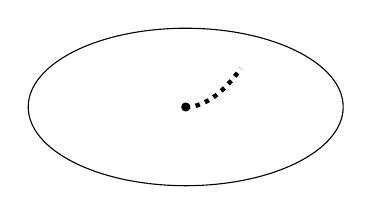
\begin{tikzpicture}
    %\node (name) at (pos1, pos2) [label={text1}] {text2};
    %\draw [option] ...;
    \draw (0,0) ellipse (2 and 1);
    \filldraw (0,0) circle (.05);
    \draw [ultra thick, dotted, domain=0:0.7] plot (\x, {(\x)^2});
    \end{tikzpicture}
\end{center}
\end{tcolorbox}

\begin{tcolorbox}
\begin{itemize}

    \item Définitions
      \begin{itemize}

          \item Espace complet, espace de Banach 
          \item Séries absolument convergentes

      \end{itemize}

    \item Théorèmes 
      \begin{itemize}

          \item Un espace compact est complet 
          \item Espace de Banach 
          \item Point fixe 
          \item Séries et espaces de Banach

      \end{itemize}

\end{itemize}
\end{tcolorbox}
\newpage

\section{Espace complète}

\subsection{Suites de Cauchy}

Un \textbf{trou} dans espace, qu'est-ce que c'est ?

Par exemple, $E = ]0, 1]$ avec  $|.|$ le valeur absolue.  $u_n = 1 / (n+1) \to 0$ dans $\mathbb{R} $ mais n'a pas de limite dans $E$.

Comment reconnaître ce type de suites ?

\begin{Definition}[colbacktitle=red!75!black]{Suite de Cauchy}{}
Soit $(E, d)$ un espace métrique,  $(u_n)_{n\in \mathbb{N} }\in E^{\mathbb{N} }$ est dite \textbf{suite de Cauchy} si :
\begin{center}
Les termes de la suite sont très procher les uns des autres.
\end{center}

\[
    d(u_p, u_q) \underset{p,q \to +\infty}{\longrightarrow} 0
\]

Asymptotiquement :
\[
    \forall \varepsilon \in \mathbb{R} _+^{*}, \; \exists N \in \mathbb{N} ,\; \forall (p,q) \in \mathbb{N} ^{2}, \; [p \ge q \ge N] \implies [d(u_p, u_q) \le \varepsilon]
\]

\end{Definition}

\begin{Prop}{Bornée d'une suite de Cauchy}{}
Toute suite de Cauchy est bornée.
\end{Prop}
\begin{myproof}
    Posons $R = \max(d(u_0, u_N),\;, \dots, d(u_{N-1}, u_{N}), \varepsilon)$, $u_n \in BF_d (u_N, R)$
\end{myproof}

\subsection{Convergence d'une suite de Cauchy} % (fold)
\label{sub:Convergence d'une suite de Cauchy}

% subsection  (end)
Une \textbf{suite de Cauchy} peut converger vers
\begin{itemize}
    \item un élément de $E$ 
    \item un \textit{trou} de $E$ (un élément qui est \textit{en dehors de} $E$)
\end{itemize}



\begin{Prop}{Suite convergente et suite de Cauchy}{}
\begin{itemize}
    \item Toute suite convergente est de Cauchy.
    \item Soit $u$ une suite de Cauchy, alors :  
      \begin{center}
          $u$ est \textbf{convergente} si, et seulement si, $\mathrm{Adh} (u) \ne \emptyset$.
      \end{center}
\end{itemize}
\end{Prop}

\begin{myproof}
\begin{itemize}
    \item Si $u_n \to \lambda$, donc $d(u_p, u_q) \le d(u_p, \lambda) + d(\lambda, u_q)$
    \item Dans deux sens :
        \begin{itemize}
            \item  $(\implies)$ Évident.
            \item $(\impliedby)$ Existence d'une sous-suite $u_{\varphi(n)}\to \lambda$ et $d(u_n,\lambda) \le d(u_{\varphi(n)}, \lambda) + d(u_n,u_{\varphi(n)})$
        \end{itemize}
\end{itemize}
\end{myproof}

\begin{note}
Pour montrer une suite de Cauchy est convergente, trouver une valeur d'adhérence.

Con convergence : Essayer de trouver un trou dans l'espace.
\end{note}
\begin{Prop}{Suite de Cauchy dans $\mathbb{R}$}{}
Toute suite de Cauchy \textit{à valeurs réelles} est convergente.
\end{Prop}
\begin{myproof}
Bornée donc d'après le théorème de Bolzano-Weierstrass (toute suite \textit{réelle bornée} admet une valeur d'adhérence), $\mathrm{Adh} (u) \ne \emptyset$.
\end{myproof}

\begin{Example}{Suites de Cauchy non convergente}{}
\begin{itemize}
    \item Cas métrique : Dans $(\mathbb{Q}, |.|)$, $$u_n = \frac{E(10^{n}\sqrt{2} )}{10^{n}}$$ est une suite de Cauchy mais n'est pas convergente dans $\mathbb{Q}$. ($\sqrt{2} \not\in \mathbb{Q} $, convergence vers un élément s qui n'est plus dans cet ensemble)

        En fait, $\mathbb{Q} $ plein de trous avec tous les éléments de $\mathbb{R} \backslash \mathbb{Q} $.

      \item Cas normé : Dans $E = \mathrm{Vect} (\{x \mapsto x^{k}, k \in\mathbb{N} \})$ (l'ensemble des fonctions polynomials) muni de $\|P\|_{\infty}= \max(|a_c|, c\in [\![0, \mathrm{deg}(P)]\!])$, la suite $(P_n)_{n\in\mathbb{N} }$ définie par :

        \[
        P_n = \sum_{k=0}^{n} \frac{1}{k!} . (x \mapsto x^{k})
        \]
        
    est une suite de Cauchy mais n'est pas convergente dans $E$.
        
\end{itemize}
\end{Example}

\begin{myproof}
\begin{itemize}
    \item Suite de Cauchy :\[
     \| P_p - P_q  \| _{\infty} =  \| \sum_{n=q+1}^{p} \frac{1}{n!} x \mapsto x^{n} \| _{\infty} \le  \frac{1}{(q+1)!}  \to 0
    \]
\item Pas de limite : Supposons que $P_n \to Q \in E$, alors $Q$ a un degré $d$. Si  $n>d$, $n \to +\infty$
     \[
     \| P_n - Q  \| _\infty \ge  \frac{1}{(d+1)!}  \not\to 0
    \]
\end{itemize}
\end{myproof}

\subsection{Espace complet, Espace de Banach}
\begin{Definition}[colbacktitle=red!75!black]{Espace complet, Espace de Banach}{}
\begin{itemize}
    \item Un espace $(E,d)$ est dit \textbf{complet} si :
      \begin{center}
        \textit{Toute} suite de Cauchy est convergente.
      \end{center}
    \item Un espace $(E,N)$ est dit \textbf{de Banach} si :
      \begin{center}
          L'\underline{espace vectoriel normé} $(E,N)$ est \textbf{complet}.
      \end{center}
\end{itemize}
\end{Definition}

\begin{Example}{$\mathbb{K}$ et espace compact}{}
\begin{itemize}
  \item $(\mathbb{K}, |.|)$ est complet.
  \item Si $(E,d)$ est compact, il est complet.
\end{itemize}
\end{Example}

\begin{myproof}{}{}
\begin{itemize}
  \item $\mathbb{R}$ déjà fait.
  \item $z_n = x_n + iy_n$, et bornée + Bolzano-Weierstrass.
  \item Par définition, tout suite d'un compact admet une valeur d'adhérence.
\end{itemize}
\end{myproof}

\begin{note}{Comment montrer qu'un espace $E$ est complet ?}{}
\begin{itemize}
  \item On prend une suite de Cauchy dans $E$, $(u_n)_{n \in \mathbb{N}} \in E ^\mathbb{N}$
  \item On construit la limite de cette suite dans un espace \textit{plus gros} $F$, avec \textit{la même norme} : $u_n \to u \in F$
  \item Montrer la convergence dans l'espace plus gros.
  \item On montre que la limite est dans cet espace. $u \in E$
    \begin{itemize}
      \item L'espace $E$ est fermé ?
      \item Connection avec des espaces complet qu'on connaît ?
    \end{itemize}
\end{itemize}

Comment montrer qu'un espace $E$ n'est pas complèt ?
\begin{itemize}
  \item On prend un élément de l'espace plus gros mais pas dans $E$
  \item On construit une suite de $E$ qui converge vers cet élément dans l'espace plus gros. 
  \item \textit{Ou bien } une suite est de Cauchy, on montre qu'elle ne converge pas.
\end{itemize}
\end{note}

\begin{Example}{Espaces de fonctions continues}{}
  Notant $I = [a, b]$,
\begin{enumerate}
  \item $E = \mathscr{C}(I, \mathbb{R}), \| .\|_{\infty, I}$ est complet. (Banach)
  \item $E = \mathscr{C}(I, \mathbb{R}), \| .\|_{1, I}$ n'est pas complet.
\end{enumerate}
\end{Example}

\begin{myproof}{}{}
\begin{enumerate}
  \item Par étape :
    \begin{itemize}
      \item Soit $(f_n)_{n \in \mathbb{N}} \in E^{\mathbb{N}}$  de Cauchy. 
      \item Pour tout $x \in I$, $(f_n(x))_{n \in \mathbb{N}}$ est une suite réelle de Cauchy car :
        \[
          |f_p(x) - f_q(x) | \le \| f_p - f_q \| _{\infty, [a,b]}
        \]
        
        Or $(\mathbb{R}, |.|)$ est complet, donc il existe un réel noté $f(x)$ tel que $f_n(x) \underset{n \to +\infty}{\longrightarrow} f(x)$. (Attention : $f \in F = \mathscr{F}(I, \mathbb{R})$ contenant $E$, on ne sait pas si $f$ est continue)

      \item Sur $F$ on peut avoir une notion de suite convergente définie par $f_n \underset{n \to +\infty}{\longrightarrow} f$ si 
        \[
          \delta_n = \mathrm{sup} _{x \in [a,b]} |f_n(x) - f(x) | \to 0
        \]

      $\delta_n \underset{n \to + \infty}{\longrightarrow} 0$ car lorsque on fait tendre $p$ vers $+ \infty$ dans l'écriture $(f_n) _{n \in \mathbb{N}}$ une suite de Cauchy, on a montré :
      \[
        \forall \varepsilon \in \mathbb{R}_+^*, \exists N \in \mathbb{N}, \forall n \in \mathbb{N}, [n \ge N] \implies \forall x\in [a,b], |f(x) - f_n(x) | \le \varepsilon
      \]

      \item Montrons que $f \in E$.

        Soit $\alpha \in [a, b]$, $h \in \mathbb{R}$, $\alpha+h \in [a,b]$, alors : $\forall \varepsilon \in \mathbb{R}+^*$, $\exists \eta >0$, si $|h| < \eta$,
        \[
          |f(\alpha+h) - f(\alpha)| \le |f(\alpha+h) - f_n(\alpha+h)| + | f_n(\alpha+h) -f_n(\alpha) | + |f_n(\alpha) - f(\alpha)| \le 3\varepsilon
        \]
        Ce qui montre la continuité en $\alpha$.

        Donc, $f\in E$ et $\delta_n  = \| f_n - f \| _{\infty, [a,b]}\to 0$.
    \end{itemize}
  \item On prend $[a,b] = [0,1]$, supposons que $f:[0,1]\to \mathbb{R},\; x \mapsto 1$ si $x\in [0, 1/2]$ et $x \mapsto 0$ sinon. On construit la suite de fonctions comme : 
    \begin{align*}
      f_n : [0, 1] &\to \mathbb{R} \\ 
            x &\mapsto \begin{cases}
              1, \; x \in \left[0, \frac{1}{2}\right] \\ 
              0, \; x \in \left[\frac{1}{2} + \frac{1}{n} , 1\right]\\ 
              n\left( \frac{1}{2} + \frac{1}{n} - x\right), \; \text{sinon}
            \end{cases}
    \end{align*}
\begin{figure}[H] %h:当前位置, t:顶部, b:底部, p:浮动页
  \centering
  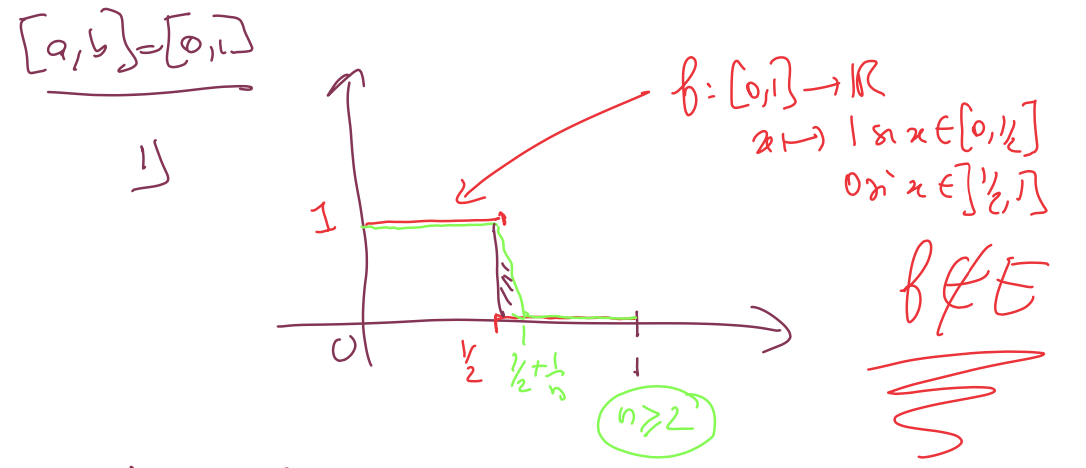
\includegraphics[width=0.9\textwidth]{./assets/Preuve-fn-f.png}
  \caption{Preuve-$f_n \to f$}
  \label{fig:Preuve-fn-f}
\end{figure}
\begin{itemize}

  \item Convergence dans $\mathcal{C} _{pm} ([0,1], \mathbb{R})$
\[
  \| f - f_n \| _{1, [0,1]} = \int _0 ^{1} |f(t) - f_n(t) | \mathrm{d} t = \frac{1}{2n}  \underset{n \to + \infty}{\longrightarrow}  0
\]
donc dans $\mathcal{C } _{pm} ([0,1], \mathbb{R})$, $f_n \underset{n \to + \infty}{\longrightarrow} f$.

\item Non convergence dans $\mathcal{C}([0,1],\mathbb{R})$

  Supposant que $f_n \underset{n \to + \infty}{\longrightarrow} g \in E$, alors 
  \[
    \int _0 ^{1} |f(t) -g(t) | \mathrm{d} t \le \int_{0}^{1}|f(t) - f_n(t) | \mathrm{d} t + \int_{0}^{1} | f_n(t) - g(t) | \mathrm{d}t
  \]

  Donc $\int_{0}^{1} |f(t) - g(t)| \mathrm{d} t = 0$, on en déduire que $(f-g)(t) = 0$ si $f-g$ continue en $E$.
  
  Mais, $g$ continue sur $[0,1]$ et $f$ continue sur $[0,1] \backslash \{1/2\}$, il contradit la continuité de $g$ car 
  \[
    g \left( \frac{1}{2} ^{-} \right) = f \left( \frac{1}{2} ^{-} \right) = 1, \quad
    g \left( \frac{1}{2} ^{+} \right) = f \left( \frac{1}{2} ^{+} \right) = 0
  \]

\end{itemize}


    
\end{enumerate}
\end{myproof}

\begin{Prop}{}{}
Un sous-ensemble \underline{fermé} d'un espace complet est lui-même complet.
\end{Prop}

\begin{myproof}{}{}
Si $F$ un fermé dans un espace complet $E$, soit $(x_n) _{n \in \mathbb{N}}$ une suite de Cauchy de $F$. 

\begin{itemize}

    \item $(x_n)$ est une suite de Cauchy de $E$, donc elle converge vers $\lambda \in E$.

    \item $F$ est fermé dans $E$, donc $\lambda \in F$.
\end{itemize}
\end{myproof}



\begin{Prop}{}{}
  Si $E'$ espace de Banach, ($\mathscr{LC}(E, E'), \vert\vert\vert . \vert\vert\vert _{N, N'})$ est aussi un espace de Banach.
\end{Prop}

\begin{myproof}{}{}
  Rappel : Si $(E, N)$ et $(E', N')$ deux espaces vectoriels normés. Soit $u\in \mathscr{L}(E, E')$
 
  \begin{itemize}
    \item $u$ est continue ssi $\exists K \in \mathbb{R} _ +$, $\forall x\in E$, $N'(u(x)) \le K.N(x)$ et ssi $u$ est continue en $0_E$.
    \item On note $\mathscr{LC}(E, E') = \{ u \in \mathscr{L}(E, E'),\; u \text{ continue}\}$
    \item On munit cet espace vectoriel de 
      \[
        \vert\vert\vert u\vert\vert\vert _{N, N'} = \underset{x \ne 0}{\mathrm{sup}} \left( \frac{N'(u(x))}{N(x)} \right) = \underset{x,N(x) = 1}{\mathrm{sup}}(N'(u(x)))
      \]
  \end{itemize}
  Soit $(u_n) _{n \in \mathbb{N}}\in \mathscr{LC}(E, E')$ une suite de Cauchy pour la norme. 

  \begin{itemize}

      \item \underline{Construction de la limite + Verification que la suite converge dans un espace plus gros}

        On a 
        \[
          \forall (p,q) \in \mathbb{N} ^{2}, \; \forall x\in E, \; N'(u _p (x) - u _q (x) ) \le \vert\vert\vert u_p - u_q\vert\vert\vert _{N, N'} N(x)
        \]

        On sait que $E'$ est complet, donc $(u_n(x)) _{n \in \mathbb{N}}$ converge, notons $u(x)$ sa limite. 

        On peut trouver $N \in \mathbb{N}$ tel que pour tout $p \ge \mathbb{N}$ et $q \ge \mathbb{N}$ :
        \[
          \vert\vert\vert u_q -u_p \vert\vert\vert _{N, N'} \le \varepsilon \implies \forall x\in E, \; N'(u_q(x) - u_p(x)) \le \varepsilon N(x) 
        \]

       Donc, comme $u_q(x) \underset{q \to + \infty}{\longrightarrow} u(x)$
       \[
          \forall x\in E, \; N'(u(x) - u_p(x)) \le \varepsilon N(x)
       \]

       (On n'a pas encore montré que $u \in \mathscr{LC}(E, E')$ !!)
     \item \underline{Verification que la limite dans $E$}

       $u$ est linéaire, puisque $u_n$ le sont.

       $u$ est continue, car elle est lipschitzienne au voisinage de $0_E$ : 
       \[
        \forall x\in E, \; N'(u(x))\le N'(u(x) - u_p(x)) + N'(u_p(x)) \le (1 + \vert\vert\vert u_p \vert\vert\vert)N(x)
       \]


  \end{itemize}
\end{myproof}



\begin{Prop}{}{}
Tout espace vectoriel normé de \underline{dimension finie} est complet.
\end{Prop}


\begin{myproof}{}{}
On passe aux coordonnées, la suite de Cauchy est bornée, et en même temps les Boules fermés sont compacts. \underline{C'est inutile de dire un espace complet en dimension infinie, utliser les notions de \textbf{compacité}.}
\end{myproof}



\newpage

\section{Théorèmes}


\subsection{Théorème de Point Fixe}

Caractérisation séquentielle des application continues. 

\begin{Prop}{Image par application continue ou uniformément continue d'une suite de Cauchy}{}
  Soit $f : (E,d) \to (E', d')$ une fonction. Si $f$ est \underline{uniformément continue}, alors, si $(x_n)_{n \in \mathbb{N}} \in E ^{ \mathbb{N}}$ est une suite de Cauchy, alors :
\begin{center}
  $(f(x_n))_{n \in \mathbb{N}}$ est une suite de Cauchy de $E'$
\end{center}

Mais, si $f$ est seulement continue, l'image par $f$ d'une suite de Cauchy n'est pas nécessairement une suite de Cauchy.
\end{Prop}

\begin{myproof}{}{}
Rappel : Définition d'\textbf{uniformément continue} :
\[
  \forall \varepsilon >0, \; \exists \delta >0, \; d(x, y) \le \delta \implies d'(f(x), f(y)) \le \varepsilon
\]
\end{myproof}

\begin{Example}{Contre-Exemple}{}
On prend :
\[
  E = ]0, 1],\quad x_n = \frac{1}{n+1} , \quad f : x \mapsto \frac{1}{x}
\]
\begin{itemize}

    \item $x_n$ est de Cauchy dans $E$, car elle converge donc suite de Cauchy dans $\mathbb{R}$. 

    \item $f$ est continue.
\end{itemize}

On obtient $f(x_n)= n+1$ qui n'est pas une suite de Cauchy dans $E$
\end{Example}




\begin{Theorem}{\color{red} Point fixe}{}
  Soit $(E, d)$ un espace \underline{complet} et $f$ une application de $E$ dans $E$ \underline{contractante}, alors : 
  \begin{center}
Il \underline{existe} un \underline{unique} \textit{point fixe} de $f$ sur $E$.
  \end{center}
\[
  \forall (x, y) \in E ^{2}, \; {\color{red} \exists k \in ]0, 1[}, \; d(f(x),f(y)) \le k d(x, y) \implies \boxed{\exists ! a \in E,\; f(a) =a}
\]
Cela aussi implique que, pour tout $a \in E$, la suite $(u_n)_{n\in \mathbb{N}}$ définie par $u_0=a,\; \forall n \in \mathbb{N}, \; u _{n+1} = f(u_n)$ vérifie $u_n\underset{n \to + \infty}{\longrightarrow} \alpha$.
\end{Theorem}

\begin{note}{}{}



Ce théorème nous donne : 

\begin{itemize}
    \item L'existence de $\alpha \implies$ permettre d'assurer que certains objets qui nous interessent ont un sens.
    \item un algorithme pour calculer $\alpha \implies$ dans suites et séries, résoudre des équations $g(x)=0$ où $g$ continue.
\end{itemize}

Utilisation : On veut montrer l'existence d'un objet mathématique $\implies$ On transforme le problème d'existence en la recherche d'un point fixe pour une fonction contractrante dans un espace complet.

\end{note}


\begin{myproof}{}{}
\begin{itemize}

    \item \underline{Existence}

Soit $u_0 = a$, $u _{n+1} = f(u_n)$, on va montrer que cette suite est de Cauchy.

Soit $(p,q) \in \mathbb{N} ^{2}$, $q>p$, 
\begin{align*}
  d(u_p, u_q) &\le \sum_{j=p}^{q-1} d(u_j, u _{j+1}) \quad \text{ Inégalités triangulaires } \\
              &\le \left( \sum_{j=p}^{q-1} k ^{j}\right) . d(u_0, u_1)\\
              &\le \frac{k ^{p}}{1-k} d(u_0, u_1)  \underset{p \to + \infty}{\longrightarrow} 0
\end{align*}

Donc $(u_n)_{n\in \mathbb{N}}$ de Cauchy dans $E$, elle converge vers $\alpha\in E$. 

Comme $f$ est continue, $f(u_n)  \underset{n \to + \infty}{\longrightarrow} f(\alpha)$, donc en passant à la limite dans la relation : $u _{n+1} = f(u_n)$ que $\alpha = f(\alpha)$, $\alpha$ est un point fixe. 

\item \underline{Unicité}

Si $f(\alpha) = \alpha$, $f(\beta) = \beta$, alors $d(\alpha, \beta) = d(f(\alpha), f(\beta) )\le kd(\alpha, \beta)$. Sachant que $k <1$, $d(\alpha, \beta)=0$ donc $\alpha=\beta$.
\end{itemize}
\end{myproof}

\begin{Prop}{\textbf{Application} : Suites et Séries}{}
Soit $g : \mathbb{R} \to \mathbb{R}$ continue et qui possède un point d'annulation $\alpha$.

Idée principal : Supposons que 
\begin{align*}
  f : \mathbb{R} &\to \mathbb{R} \\
  x &\mapsto x + \lambda.g(x)
\end{align*}
et trouver $\lambda \in \mathbb{R}$ tel que $f$ soit contractante.
\end{Prop}
\begin{Example}{Application}{}
On cherche à montrer l'existance d'une solution de l'équation différentielle :
\[
\begin{cases}
    y' = \psi (x, y) \\
    y(x_0) = y_0
  \end{cases} \text{ où } \psi : O \subset \mathbb{R}^{2} \to \mathbb{R} \text{ continue }
\]
\end{Example}

\begin{myproof}{}{}
Si $\varphi$ est une solution, c'est-à-dire : $\begin{cases}
  \varphi'(x) = \psi(x, \varphi(x)) \\ \varphi(x_0) = y_0
\end{cases}$ alors :

\begin{itemize}

    \item Pour tout $x \in D_f( \varphi)$, 
\[
  \varphi(x) = \varphi(x_0) + \displaystyle\int_{x_0}^{x} \psi(t, \varphi(t)) \mathrm{d}t
\]

\item (De $f(\varphi(x)) = \varphi(x)$, on obtient) \underline{$\varphi$ est un point fixe de l'application} $f : \varphi \mapsto \left(x \mapsto y_0+ \int_{x_0}^{x}\psi(t, \varphi(t) )\mathrm{d}t \right)$.

\item Sous l'hypothèse $\varphi$ de classe $\mathcal{C} ^{1}$, on peut trouver $\mathcal{V}_{x_0}$ voisinage de $x_0$, et un $E = \{g \in \mathcal{C}( \mathcal{V} _{x_0}, \mathbb{R}), g(x_0)=y_0\}$. Si $\mathcal{V}_{x_0}$ est \textbf{compact}, $(E,d)$ est complet.
\item Si on prend $V _{x_0}$ assez petit, on montre que $f$ est contractante. C'est-à-dire, on veut montrer que $\forall (x_1, x_2) \in \mathcal{V} _{x_0} ^{2}$, $\| f(\varphi(x_1)) - f(\varphi(x_2)) \| _{\infty} \le k |x_1 -x_2 |$. 

  \begin{align*}
    |f(\varphi(x_1) ) - f(\varphi(x_2)) | &= | \int _{x_1} ^{x_2} \psi(t, \varphi(t)) \mathrm{d} t | \\ 
                                          &\le |x_1 -x_2 | \underset{t \in \mathcal{V} _{ x_0}}{\mathrm{sup}} |\psi(t, \varphi(t))|
  \end{align*}

  Si $\mathcal{V} _{x_0}$ assez petite, $|x_1 -x_2|$ assez petit et $|\psi(t, \varphi(t)| \le M$ est bornée.

  Comme $y(x_0) = y_0$, $\psi(x_0, y_0) =0$ donc au voisinage de $x_0$, $\psi(t, \varphi(t)) \le \varepsilon$.


\item Donc, il existe un unique point fixe $\varphi_0$ et $\forall x \in \mathcal{V}_{x_0}$, $\varphi_0(x) = y_0 + \int _{x_0} ^{x} \psi (t, \varphi_0(t)) \mathrm{d}t$. D'après TFA, $\varphi_0$ est de classe $\mathcal{C} ^{1}$ et vérifie les conditions sur $\mathcal{V} _{x_0}$, on a trouvé une solution avec $\varphi_0 \in \mathcal{C}^{1}$.
\end{itemize}



\end{myproof}

\subsection{Séries et espace de Banach} % (fold)
\label{sub:Séries et espace de Banach}

% subsection Séries et espace de Banach (end)

\begin{Definition}[colbacktitle=red!75!black]{Séries absolument convergentes}{}
Soit $(E,N)$ espace vectoriel normé, et $\sum_{}^{}x_n$ une séries à termes dans $E$.

$\sum_{}^{}x_n$ est \textbf{absolument convergente} si :
\center 
La séries à termes réels positifs $\sum_{}^{} N(x_n)$ est convergente.
\end{Definition}

\begin{Theorem}{Séries et espace de Banach}{}
Soit $(E, N)$ espace vectoriel normé. 

\center 
$(E,N)$ est un \textbf{espace de Banach} si et seulement si toute séries \textbf{absolument convergente} d'éléments de $E$ est \underline{convergente} dans $E$.
\end{Theorem}


\begin{myproof}{}{}
  (...)
\end{myproof}




\subsection{Prolongement des applications uniformément continues}

Rappel : \textbf{Théorème des prolongement $\mathcal{C} ^{1}$}
Soit $f : [a, b[ \to \mathbb{R}$ de classe $\mathcal{C} ^{1}$.  Si $f'(t)  \underset{t \to b ^{-}}{\longrightarrow} l$ alors : 
\begin{itemize}

    \item $f$ admet une limite $\alpha$ en $b ^{-}$ 
    \item La fonction $\widetilde{f} : [a,b] \to \mathbb{R}$ est de classe $\mathcal{C} ^{1}$ :
      \begin{align*}
        \widetilde{f} : [a,b] &\to \mathbb{R} \\ 
        t &\mapsto \begin{cases}
          f(t), \quad t \in [a,b[ \\ 
          \alpha, \quad t = b
        \end{cases}
      \end{align*}

\end{itemize}

\begin{note}{}{}
Pour prolonger $f \in \mathcal{C} ^{1}$, on n'a pas besoin que \underline{$f'$ ait une limite}. 
\end{note}

\[
  f(x) = f(a) + \int_{a }^{x } f'(t) \mathrm{d} t, \quad x \in [a, b[
\]

Comme $f'(t)  \underset{ t \to b ^{- }}{\longrightarrow} l$, $\int_{a }^{x } f'(t) \mathrm{d} t  \underset{x \to b ^{- }}{\longrightarrow} \int_{a }^{b } f'(t) \mathrm{d}t$
\[
  f(x)  \underset{ x \to b ^{-}}{\longrightarrow} f(a) + \int_{a }^{b } f'(t) \mathrm{d} t = \alpha
\]

Ici, $f'$ bornée sur $[a, b[$, $f$ est lipschitzienne (TAF), donc $f$ est \textbf{uniformément continue}. 

\begin{Theorem}{Prolongement des applications uniforméments continues}{}
  Soit $(E, d)$ et $(E', d')$ deux espaces métriques, tels que $E'$ est \textit{complet}, soit $A \subset E$, pour une fonction $f : A \to E'$ \underline{uniformément continue}, il existe une unique fonction définie et \underline{\textit{continue} sur $\bar{A}$} telle que $$\forall a \in A, \widetilde{f} = f$$. 

  On l'appelle \textbf{prolongement} de $f$ à $\overline{A}$. 

  De plus $\widetilde{f}$ est \textit{uniformément continue} sur $\overline{A}$.
  
\[
  f: A \to E' \text{ uniformément continue } \implies \widetilde{f} : \overline{A} \to E' \text{ uniformément continue }
\]
\end{Theorem}


Remarque : 
\begin{itemize}

    \item Une application continue envoie une suite convergente sur une suite convergente (caractérisation séquentielle de la continuité)

    \item Une application \textit{uniformément continue} envoie une suite de Cauchy sur une suite de Cauchy.

\end{itemize}

\begin{Example}{Prolongements utiles}{}
\begin{itemize}

  \item \underline{Fonction réelle} : Soit $f : ]a, b[ \to \mathbb{R}$ uniformément continue, alors $f$ admet une limite en $a ^{+}$. 
  \item L'intégrale sur les fonctions \textit{continues par morceaux} sur $[a, b]$ à valeurs dans $\mathbb{K}$ est \textit{uniformément continue} comme elle est linéaire et lipschitizienne en 0 : 
    \[
      \Psi : \begin{cases}
        \mathscr{C} ^{0}_{pm} ([a,b], \mathbb{K}), \| . \| _{\infty, [a,b]} \to \mathbb{K} \\ 
        f \mapsto \int_a ^{b} f(t) \mathrm{d} t
      \end{cases}
    \]
    Elle peut se prolonger à l'adhérence de $\mathscr{C} _{pm} ^{0} ([a,b], \mathbb{K})$ pour la norme $\| . \|_{\infty, [a,b]}$ dans $\mathcal{F}([a,b], \mathbb{K})$.

\end{itemize}
\end{Example}

\begin{Prop}{Segments emboîtés (déjà vu)}{}
  Soit $I_n = [a_n,b_n]$, $\forall n \in \mathbb{N}, a_n \le b_n$, si $\forall n\in \mathbb{N}$, $I_{n+1} \subset I_n$, alors 
  \[
    \bigcap _{n \in \mathbb{N}} I_n \ne \emptyset
  \]
  de plus si  $b_n - a_n  \underset{n \to + \infty}{\longrightarrow} 0$, il existe un $\alpha \in \mathbb{R}$, $\bigcap _{n \in \mathbb{N}} I_n = \{ \alpha \}$
\end{Prop}


\begin{Theorem}{Fermé emboîtés (complète)}{}
  Soit $(E, d)$ un espace complet, $(F_n) _{n\in \mathbb{N}}$ des \underline{fermés} non vides de $E$ tels que 
\[
  {\color{red}\mathrm{diam}(F_n)  \underset{n \to + \infty}{\longrightarrow}  0} \text{ et } \forall n \in \mathbb{N},\; F _{n+1} \subset F_n
\]
Alors 
\[
  \exists ! \alpha \in E, \bigcap _{n \in \mathbb{N}} F_n = \{ \alpha\}
\]
\end{Theorem}

\begin{myproof}{}{}
  Rappel : $\mathrm{diam}(F) = \underset{(x,y) \in F ^{2} }{\mathrm{sup}} d(x, y) \in \mathbb{R} _ + \cup \{+ \infty\}$ si $F \ne \emptyset$
\begin{itemize}

    \item Existence : 
Soit $(x_n) _{n \in \mathbb{N}}$ définie par $\forall n \in \mathbb{N}$, $x_n \in F_n$. 

Cette suite est de Cauchy car pour tout $p, q$, $d(x_p,x_q) \le \mathrm{diam}(F_q)  \underset{q \to + \infty}{\longrightarrow} 0$

Cette suite converge donc vers un élément $\alpha \in E$. De plus, pour $p \in \mathbb{N}$, comme $(x_n) _{n \in \mathbb{N}, n \ge p } \in F_p ^{\mathbb{N}}$ et que $F_p$ est fermé dans $E$, $\alpha \in F_p$

\item Unicité : Évidente d'après la propriété du diamètre.

\end{itemize}
\end{myproof}



\begin{Theorem}{Baire}{}
Si $(E,d)$, alors : $\forall (O_n) _{n \in \mathbb{N}}$ \underline{ouverts denses} de $E$, $$\overline{ \bigcap _{n \in \mathbb{N} }O_n} = E$$
\end{Theorem}

\begin{myproof}{}{}
On va montrer que, pour n'importe quelle $x \in E$, et une boule ouverte de $x$, il y a toujours une intersection avec $\bigcap O_n$. 

Soit $x \in E$, soit $\varepsilon >0$, nous allons montrer que 
\[
  BO(x, \varepsilon) \cap \left(\bigcap _{n\in \mathbb{N}} O_n\right) \ne \emptyset
\]

Récurrence : 
\begin{itemize}

    \item $O_0$ est dense, donc il existe $x_0 \in BO(x, \varepsilon) \cap O_0$ (ouvert de $E$)

      Il existe alors une boule de rayon $r_0>0$ telle que $BF(x_0, r_0) \subset BO(x, \varepsilon) \cap O_0$

    \item On construit de proche en proche $(x_n, r_n) _{n \in \mathbb{N}} \in (E \times \mathbb{R} _+ ^{*}) ^{\mathbb{N}}$ telles que : 
      \[
        \forall n \in \mathbb{N} ^{*}, \; BF(x_n, r_n) \subset BO(x _{n-1}, r _{n-1}) \cap O_n, \text{ et }  r_n \le \frac{r _{n-1}}{2}
      \]

    D'après le théorème précédante, le diamètre $\le 2r_n  \underset{r \to + \infty}{\longrightarrow} 0$, il existe un point $\alpha \in E$ tel que :
    \[
      \alpha \in BO(x, \varepsilon) \cap \left( \bigcup _{n\in \mathbb{N}} O_n \right)
    \]

\end{itemize}
\end{myproof}
C'est un théorème très puissant conduisant à des résultats surprenants. 



\begin{Prop}{Conséquence du théorème de Baire}{}
Un espace complet ne peut être \underline{réunion dénombrable} de \underline{fermés d'intérieurs vides}.
\end{Prop}
\begin{myproof}{}{}
En fait, $O$ ouvert dense $\iff$ $O ^{c}$ fermé d'intérieur vide :
\[
  \dot{\overline{O ^{c}}} = \bar{O} ^{c} = E ^{c} = \emptyset; \quad \overline{O} ^{c} = \dot{\overline{O ^{c}}} = \dot{\emptyset} = \emptyset
\]
\end{myproof}

\begin{Example}{Utilisation du théorème}{}
  \underline{Fonction polynomiales} : $(\mathrm{Vect}(\{x \mapsto x ^{n}, n \in \mathbb{N}\}, N)$ n'est jamais complet, quelle que soit $N$.
\end{Example}

\begin{myproof}{}{}
  Soit $E_n =\mathrm{Vect}(\{x \mapsto x ^{k},\; k \in [\![0,n]\!]\})$ fonctions polynomiales de degré $\le n$. $E = \bigcup _{n\in \mathbb{N}} E_n$. 
  \begin{itemize}

      \item $E_n$ fermé dans $E$ (de dimension finie)
      \item $\dot E_n = \emptyset$ car si $x \in \dot E_n$, il existe $\varepsilon >0$, $BO(x, \varepsilon) \subset E_n$, alors $\mathrm{Vect}(BO(x,\varepsilon) \subset E_n$, mais $\mathrm{Vect}(BO(x,\varepsilon))$ est toujours $E$. (Voir proposition suivant) Contradiction.
  \end{itemize}
\end{myproof}

\begin{Prop}{}{}
  Dans un espace vectoriel normé, toute \underline{boule ouverte non vide} est une \underline{partie génératrice}. 
\end{Prop}

\begin{myproof}{}{}
Soit $(E,N)$, $B = BO(x_0, r)$, $E_1 = \mathrm{Vect}(B)$. On a 
\begin{itemize}

    \item $BO(0_E, r) \subset E_1$. 

      Si $x \in BO(0_E, r)$, $x + x_0 \in BO(x_0, r) \subset E_1$, de plus $x_0 \in E_1$ donc $x \in E_1$
    \item $E_1 = E$, soit $x \in E \backslash \{0_E\}$, donc 
      \[
        \frac{r}{2N(x)}.x \in BO(0_E, r) \subset E_1 \implies x\in E_1
      \]

\end{itemize}
\end{myproof}






\begin{Definition}[colbacktitle=red!75!black]{Espace de Baire}{}
La définition $\forall (O_n) _{n \in \mathbb{N}}$ ouverts denses, $\overline{\bigcap O_n} = E$ est une définition ne faisant pas intervenir la distance donc on peut s'utiliser quand on n'a pas de distance. 

On la note \textbf{espace de Baire}. 
\end{Definition}





